\documentclass[a4paper,12pt]{article}
\pagestyle{plain}
\usepackage[T1]{fontenc}
\usepackage[latin1]{inputenc}
\usepackage[ngerman]{babel}
\usepackage{graphicx}
\usepackage{amsmath}
\usepackage{amsfonts}
\usepackage{bbm}
  
\usepackage{amssymb}
\hoffset=-1in   % Korrektur des idiotischen Standard-Offsets
\voffset=-1in   % Korrektur des idiotischen Standard-Offsets
\topmargin=1cm
\textheight=24cm
\oddsidemargin=3cm
\textwidth=15cm 
\frenchspacing
\usepackage{palatino}
\usepackage{listings}
\usepackage[T1]{fontenc}
\usepackage{babel}

 

\begin{document}
\title{\vspace{30mm} \bf{Titel}}
\author{Thomas Fischbach}
\date{\today}
\maketitle

\vfill
  
  
  
  
\tableofcontents  
  
\newpage
  
\section{Einleitung}
In der Arbeitsgruppe LARISSA\footnote{\textbf{La}ser \textbf{R}esonance
\textbf{I}onisation \textbf{S}pektroscopy for \textbf{S}elective Tracer
\textbf{A}nalysis} des Instituts für Physik an der Johannes Gutenberg
Universität Mainz wurden über viele Jahre hinweg Methoden zur
Resonanzionisations-Massenspektrometrie (RIMS) entwickelt und verbessert.
Mithilfe dieser Methoden wurden in der Vergangenheit empfindliche und selektive
Ultraspurenbestimmungen verschiedener Elemente der seltenen Erden sowie
vorrangig der radiotoxischen Actinoide durchgeführt. Voraussetzung für die
Ultraspurenanalyse dieser Elemente ist eine möglichst hohe Isotopen- und Isobarenselektivität, welche durch Kombination von elementselektiver resonanter Laserionisation und
isotopenselektiver Quadrupolmassenspektrometrie (QMS) realisiert wird.
Zur Laserionisation werden dabei in der Arbeitsgruppe zwei verschiedene Lasersysteme verwendet, zum einen
gepulst betriebene Titan:Saphir-Laser und zum anderen Kombinationen aus
Dauerstrich-Diodenlasern.\par
Ein wichtiges Teilgebiet dieser Untersuchungen befasst sich mit der
hochauflösenden Ultraspurenanalyse von Uranisotopen (siehe
Nuklidkartenausschnitt Abb.
\ref{fig:uran_nuklidkarte}) mittels HR-RIMS\footnote{\textbf{H}igh
\textbf{R}esolution-RIMS}.
\begin{figure}[h]
 	\centering
 	\fbox{\parbox{\dimexpr \linewidth - 2\fboxrule - 2\fboxsep}{
 	\centering
	    \includegraphics[width=\textwidth-5cm]{gfx/uran_nuklidkarte}
	}}
	\caption[Gesamter experimenteller Aufbau,
	schematisch]{Ausschnitt der Karlsruher Nuklidkarte für langlebige
	Uranisotope \cite{nuklidkarte}.}\label{fig:uran_nuklidkarte}
\end{figure}
Das Schwermetall Uran ist das schwerste natürlich vorkommende Element auf der
Erde mit den beiden dominanten quasi-stabilen Isotopen $^{238}$U und $^{235}$U.
Da $^{238}$U und $^{235}$U in der Natur nicht aus anderen Elementen nachgebildet werden können, lassen sich aus dem durch die Lebenszeiten ermittelbaren natürlichen Isotopenverhältnis
$\nicefrac{^{235}\text{U}}{^{238}\text{U}}=0,00725$ Rückschlüsse auf die
Entstehungszeit unseres Sonnensystems ziehen. Das dritte quasi-stabile Isotop $^{234}$U resultiert aus
$\alpha$-$2\beta$-Zerfällen von $^{238}$U. Das weitere langlebige Isotop
$^{236}$U entsteht durch Einfang thermischer Neutronen aus $^{235}$U. Im
natürlichen Gleichgewicht resultieren Isotopenverhältnisse von
$\nicefrac{^{236}\text{U}}{^{238}\text{U}}=10^{-14}$ aus Neutronenflüssen der
kosmischen Strahlung \cite{Richter1999}. Da in Kernreaktoren sehr hohe
Neutronenflüsse herrschen, können dort wesentlich höhere
$\nicefrac{^{236}\text{U}}{^{238}\text{U}}$-Isotopenverhältnisse bis hinauf zu
$1,4\cdot10^{-4}$ erzielt werden. Die Abweichung vom natürlichen Verhältnis kann
also als Referenz dienen, um einen anthropogenen Eintrag von Uran in die Umwelt nachzuweisen.\par
Eine Obergrenze für die unbedenkliche Aufnahmerate von Uran liegt
bei $0,6\,$\textmu g pro Tag und kg Körpergewicht, wobei das Grund- bzw.
Trinkwasser mit $10^{-6}\,\nicefrac{\text{g}}{\text{l}}$ belastet ist
\cite{who:2005}. Die Überhöhungen der natürlichen Verhältnisse von 
$\nicefrac{^{236}\text{U}}{^{238}\text{U}}$ resultieren maßgeblich aus
Nuklearwaffentests bis einschließlich 1998 und nicht zuletzt aus Reaktorunfällen
wie der bekannte "`Tschernobyl-Unfall"' oder der aktuell brisante Unfall in
Fukushima, Japan. Da die Kontamination der Umwelt großflächig verteilt und stark
verdünnt sein kann, ist es notwendig, sehr kleine Isotopenverhältnisse messen zu
können. Die HR-RIMS bietet hierfür hervorragende Möglichkeiten. Die große
Wichtigkeit dieses Nachweises ist in der Tatsache begründet, dass die Aufnahme von Uran in den Körper toxisch
wirkt und durch die kurzlebigen Uranisotope eine erhöhte Strahlenbelastung
gegeben ist.\par
Um mithilfe von Lasern nicht nur elementselektiv, sondern auch
isotopenselektiv ionisieren zu können\footnote{Isotopieverschiebung, siehe
\ref{subsec:isotopieverschiebung}} und hochauflösende Spektroskopie zu
betreiben, wird sehr schmalbandiges Laserlicht benötigt, welches mit
Dauerstrichlasern erzeugt werden kann. Diodenlaser sind für diesen Einsatz eine
optimale und kostengünstige Lösung. Da die Übergangslinien bei Benutzung von
schmalbandigen Diodenlasern teilweise ebenfalls nur wenige MHz Breite aufweisen,
ist eine aktive Frequenzstabilisierung der Laser unabdingbar.\par
Im Rahmen dieser Diplomarbeit soll eine Frequenzstabilisierung für ein
Diodenlasersystem entwickelt und für den Einsatz zur HR-RIMS an Uran charakterisiert werden.
Folgende Anforderungen werden an das Lasersystem und die Stabilisierung gestellt:
\begin{setlength}{\leftmargini}{1cm}
	\begin{description}
		\item[Stabilität und Frequenzsicherheit]\hfill\\
			Die Laser sollen sowohl auf langen als auch kurzen Zeitskalen (wenige ms bis
			einige Stunden) stabil auf ihrer Frequenz gehalten werden. Die
			Kurzzeitstabilität wird gefordert, um laserinduzierte Zählratenfluktuationen
			zu minimieren. Dabei sind Frequenzfluktuationen von deutlich weniger als
			$10\,$MHz angestrebt. Langzeitdrifts sollen völlig eliminiert werden, um auch
			über lange Zeiten angelegte Messungen reproduzierbar durchführen zu können.
			Dabei ist es wichtig, dass die Stabilisierung ausfallsicher implementiert wird, was
			fehlerfreie Detektion von Frequenzabständen und präzise Steuerung der Laser
			voraussetzt.
		\item[gezielte Frequenzverstimmung]\hfill\\
			Um gezielt atomare Übergangsfrequenzen anfahren und spektroskopische
			Messungen durchführen zu können, soll die Möglichkeit der individuellen
			Laserfrequenzverstimmung implementiert werden. Insbesondere bei
			Isotopenverhältnismessungen ist ein regelmäßiger Wechsel der
			Anregungsschritte verschiedener Uranisotope notwendig.
		\item[Geschwindigkeit]\hfill\\
			Zur Steigerung der Messeffizienz wird angestrebt, Frequenzverstimmungen
			möglichst schnell abzuwickeln. Frequenzverstimmungen von einigen
			GHz sollen innerhalb weniger Sekunden vollzogen werden, um speziell kleine
			Probenmengen möglichst effizient nutzen zu können.
		\item[Automatisierung]\hfill\\
			Um Messungen präzise, systematisch und reproduzierbar durchführen zu
			können, soll die Steuerung der Laser - soweit möglich - vollständig
			automatisiert werden, wobei als Schnittstelle zum Experimentator ein PC mit
			einem \textit{Labview}-Programm dienen soll. Neben der Laserkontrolle soll
			auch die Messdatenaufnahme über denselben PC erfolgen.
	\end{description}
\end{setlength} 
Zur Realisierung der Laserstabilisierung wird die bewährte Methode des
\textit{Fringe-Offset-Locking} \cite{kuschnick:2000:diplomarbeit}, basierend auf
einem \textit{scanning FPI}\footnote{\textit{scanning FPI}: ein in der Länge
verstimmbares Fabry-Pérot-Interferometer}, durch eine kommerzielle
Stabilisierungstechnik, basierend auf einem festen Quadraturinterferometer,
ergänzt.\par
Der Inhalt dieser Arbeit soll die Entwicklung und den Aufbau des Lasersystems,
der optischen Komponenten der Frequenzstabilisierung inklusive Elektronik, die
Programmierung der Software zur Stabilisierung und Experimentsteuerung und die
Charakterisierung des Gesamtsystems umfassen.

\section{Theoretische Grundlagen}
Im folgenden Kapitel sollen die wichtigsten physikalischen Grundlagen für das
Verständnis der in dieser Arbeit behandelten Thematik erklärt werden. Dabei
werden die Kenntnisse über den Aufbau des Atoms, die quantisierten Lösungen der
Schrödinger- bzw. Diracgleichung, die dabei auftretenden Drehimpulskopplungen
und die daraus resultierenden Energieaufspaltungen der Atome als vorhanden
vorausgesetzt. Diesbezüglich sei auf einschlägige Lehrbücher wie
\cite{demtroeder:ex3}, \cite{demtroeder:laserspektroskopie} und \cite{saleh:grundlagen_der_photonik}
verwiesen.\\ In Kapitel \ref{sec:licht-atom-wechselwirkung} soll die Wechselwirkung von
Licht und Atom behandelt werden. Darauf aufbauend soll
in Kapitel \ref{sec:ris} die Resonanz-Ionisations-Spektroskopie,
kurz RIS, in Bezug auf die Resonanz-Ionisation von Uran-Isotopen erklärt
werden. Kapitel \ref{sec:diodenlaser} soll das Funktionsprinzip von
Halbleiterlasern und deren Rolle in diesem Projekt wiedergeben.

\section{Licht-Atom-Wechselwirkung}\label{sec:licht-atom-wechselwirkung}
Essenziell wichtig für die Resonanz-Ionisation ist das Verständnis der atomaren
Wechselwirkung mit einem elektromagnetischen Feld. Im Folgenden soll insbesondere auf die
atomaren Übergänge und deren Linienprofil eingegangen werden, da dies bei der
Atom-Spektroskopie eine wichtige Rolle spielt. Der größte Teil der dieses
Theorie-Abschnitts basiert im Wesentlichen auf den o.g. Lehrbüchern.

% $$P_{ik}=\frac{2\pi}{\hbar^2}\lvert\langle\psi_k^0\rvert\hat{\mathcal{H}}'\lvert\psi_i^0\rangle\rvert^2\delta(E_k^0-E_i^0+\hbar\omega)$$
% $$W_{ki}=\frac{\pi e^2}{3\varepsilon_0\hbar^2}\lvert\langle\psi_k\rvert\vec{r}\lvert\psi_i\rangle\rvert^2\cdot\omega_{\nu}$$
% $$B_{ki}=\frac{2}{3}\frac{\pi^2e^2}{\varepsilon_0\hbar^2}\lvert\langle\psi_k\rvert\vec{r}\lvert\psi_i\rangle\rvert^2$$
% $$\vec{M}_{ik}=e\langle\psi_i\rvert\vec{r}\lvert\psi_k\rangle$$
% $$\langle p\rangle = e\langle r\rangle = e\langle\psi_i\rvert
% r\lvert\psi_i\rangle$$
% $$\lvert\psi_k\rangle$$
% $$\bar p ^2 \rightarrow \frac{1}{2}(\lvert M_{ik}\rvert+\lvert M_{ik}\rvert)^2 =
% 2\lvert M_{ik}\rvert^2$$


\subsection{Übergangsraten}\label{subsec:uebergangsraten}
Befindet sich ein Atom in einem elektromagnetischen Feld können Absorptions- und
Emissions-Prozesse beobachtet werden. Im ersten Fall absorbiert das Atom ein
Photon einer bestimmten Mode mit der Energie $\hbar\omega_L$ aus dem elektromagnetischen Feld.
Dabei wird das Atom von einem Zustand in einen entsprechend der Photonenenergie
energetisch höher gelegenen Zustand überführt:
\begin{equation}\label{eq:uebergang}
	E_f-E_i=\hbar\omega_L
\end{equation}
Dabei ist zu beachten, dass gebundene Zustände immer quantisiert sind, also
nicht kontinuierlich im Energiespektrum verteilt sind. Analog kann ein Atom ein
Photon in das elektromagnetische Feld emittieren\footnote{Die Emission ist
auch ohne Feld möglich. Dieser Fall wird \textit{spontane Emission} genannt}.
Die Zustandsänderung des Atoms folgt dann entsprechend von einem Zustand in ein energetisch niedriger gelegenen Zustand.\par

\subsubsection{Fermis goldene Regel}\label{subsubsec:fermis_goldene_regel}
Grundlegend beschreibt \textit{Fermis goldene Regel} die
Übergangsrate von einem Zustand $\Psi_i$ (i: \textit{initial}) in einen
beliebigen Zustand $\Psi_f$ (f: \textit{final}). Diese kann halbklassisch
störungstheoretisch hergeleitet werden.  Dabei betrachtet man das externe elektromagnetische Feld als Störung
zusätzlich zum zeitunabhängigen Hamilton-Operator $\OPH_0$:
\begin{equation}\label{eq:hamilton}
	\OPH(t)=\OPH_0+\OPH'(t)
\end{equation}
mit dem Wechselwirkungsoperator
\begin{equation}\label{eq:ww}
	\begin{split}
		\OPH'(t) &= -E_0\vec{\epsilon}\cdot\OPv{d}\cos{(\vk\cdot\vr-\omega_L t)}\\
		&=
		-\OPH'\left(\mathrm{e}^{\mathrm{i}(\vk\cdot\vr-\omega_L
		t)}+\mathrm{e}^{-\mathrm{i}(\vk\cdot\vr-\omega_L t)}\right)\\
		&\text{mit}\quad
		\OPH'=\frac{1}{2}E_0\vec{\epsilon}\cdot\OPv{d}\,.
	\end{split}
\end{equation}
Hierbei ist $E_0$ die Amplitude und $\vec{\epsilon}$ der
Polarisierungsvektor des elektromagnetischen Feldes. $\OPv{d} = e\OPv{r}$ ist
der Dipoloperator. Zusätzlich kann man die Annahme machen, dass das Atom in Relation zur
Wellenlänge des Lichts sehr klein ist und es somit am Ort
des Atoms nur verschwindend geringe örtliche Änderungen der Amplitude des
elektromagnetischen Feldes erfährt ($\vk\cdot\vr\ll 1$, Atom am Ort $\vr=0$). Diese Näherung nennt man
\textit{Dipolnäherung}. Dadurch folgt für die Entwicklung des
Ortsteils der Exponentialfunktionen in erster Ordnung
$\mathrm{e}^{\pm\mathrm{i}\vk\cdot\vr}\approx1$. Nun setzt man mit der zeitabhängigen Schrödingergleichung an und entwickelt $\Psi(t)$ in die stationären Eigenzustände $\Psi_n$ des Atoms:
\begin{equation}\label{eq:sgl_stoerung_01}
	\mathrm{i}\hbar\pfrac{}{t}\ket{\Psi(t)}=\OPH(t)\ket{\Psi(t)}\,,
	\quad
	\ket{\Psi(t)}=\sum_n{c_n(t)\mathrm{e}^{-\frac{\mathrm{i}}{\hbar} E_n
	t}\ket{\Psi_n}}
\end{equation}
Führt man die Zeitableitung aus und projiziert beide Seiten der Gleichung auf
einen beliebigen Zustand $\Psi_f$, findet man
\begin{equation}\label{eq:sgl_stoerung_02}
	\dot
	c_f(t)=-\frac{\mathrm{i}}{\hbar}\sum_n{c_n(t)\mathrm{e}^{-\mathrm{i}\omega_{nf}t}\bra{\Psi_f}\OPH'(t)\ket{\Psi_n}}
	\quad\text{mit}\quad
	\omega_{nf}=\frac{E_n-E_f}{\hbar}\,.
\end{equation}
Nimmt man nun an, dass die Störung klein ist, das Atom also vornehmlich im
Ausgangs-Zustand $\Psi_i$ bleibt ($c_i(0)=1$, $c_i(t)\approx 1$, $c_{n\neq
i}\approx0$), verkürzt sich die Summe in Gl. \eqref{eq:sgl_stoerung_02}
auf einen Summanden mit $n=i\neq f$. $c_f(t)$ folgt aus zeitlicher Integration von $\dot c_f(t)$ mit
Gl. \eqref{eq:ww}:
\begin{equation}\label{eq:koeff_cf}
	\begin{split}
		c_f(t) &= \int_0^t{\dot c_f(t')\dd t'}\\
		&=
		-\frac{\mathrm{i}}{\hbar}\bra{\Psi_f}\OPH'\ket{\Psi_i}\left[\frac{\mathrm{e}^{\mathrm{i}(\omega_{fi}-\omega_L)t}-1}{\mathrm{i}(\omega_{fi}-\omega_L)}+\frac{\mathrm{e}^{\mathrm{i}(\omega_{fi}+\omega_L)t}-1}{\mathrm{i}(\omega_{fi}+\omega_L)}\right]\\
		&\text{mit}\quad
		\omega_{fi}=-\omega_{if}
	\end{split}
\end{equation}
Zu beachten ist hierbei, dass im Falle der Absorption der Nenner des zweiten
Bruchs in Gl. \eqref{eq:koeff_cf} im nahresonenten Fall
($\omega_{fi}\approx\omega_L$) in der Größenordnung $2\omega_{fi}\approx
\unit{10^{15}}{s^{-1}}$ (bei optischen Übergängen) liegt. Somit wird der
zweite Bruch verschwindend gering gegenüber dem ersten und kann vernachlässigt
werden. Im Falle der Emission betrachtet man Übergänge vom energetisch höheren
Niveau zum energetisch niedrigeren Niveau. Dabei gilt
($\omega_{if}\approx\omega_L$), wodurch der erste Bruch vernachlässigt werden
kann. Diese Näherung wird auch \textit{Rotating-Wave-Approximation} (kurz RWA)
genannt. Im Folgenden wird allerdings exemplarisch die Absorption betrachtet.\\ Für die Übergangswahrscheinlichkeit ergibt sich
\begin{equation}\label{eq:uebergangs_wkt}
	\begin{split}
		P_{i\to f}(t,\Delta\omega) &= \abs{c_f(t)}^2\\
		& =
		\frac{1}{\hbar^2}\abs{\bra{\Psi_f}\OPH'\ket{\Psi_i}}^2\cdot\frac{\sin^2{\left(\frac{\Delta\omega}{2}t\right)}}{\left(\frac{\Delta\omega}{2}\right)^2}\\
		&\text{mit}\quad
		\Delta\omega=\omega_L-\omega_{fi}\,.
	\end{split}
\end{equation}
Für die totale Übergangswahrscheinlichkeit gilt dann mit Gl.
\eqref{eq:uebergangs_wkt}
\begin{equation}\label{eq:uebergangs_wkt_total}
	\begin{split}
		P_{i\to f}(t)
		&= \int{P_{i\to f}(t,\Delta\omega)\rho(E_f)}\dd E_f\\
		&\approx \rho(E_f)\int{P_{i\to f}(t,\Delta\omega)}\dd E_f\\
		&= \hbar\rho(E_f)\int_{-\infty}^{\infty}{P_{i\to
		f}(t,\Delta\omega)}\dd(\Delta\omega)\\
		&= \frac{2\pi t}{\hbar}\rho(E_f)\abs{\bra{\Psi_f}\OPH'\ket{\Psi_i}}^2\,.
	\end{split}
\end{equation}
Hierbei wurde die Energieniveaudichte $\rho(E_f)=\fracd{n}{E_f}$ eingeführt. Sie
beschreibt die Verteilung der Energieniveaus der Endzustände $E_f$. Mit anderen
Worten: Man nimmt nicht mehr ein diskretes Endniveau an, sondern eine Kontinuum
von Endzuständen. Mit der Annahme, dass sich $\rho(E_f)$ gegenüber $P_{i\to
f}(t,\Delta\omega)$ nur langsam ändert, kann $\rho(E_f)$ in Gl. \eqref{eq:uebergangs_wkt_total} als hinreichend konstant angenommen und aus dem Integral gezogen werden. Weiterhin wurde die Substitution $\dd E_f=\hbar\dd(\Delta\omega)$ vorgenommen. Für die
totale Übergangsrate folgt dann mit Gl. \eqref{eq:uebergangs_wkt_total}
für genügend große Zeiten ($t\to\infty\stackrel{\wedge}{=}
t\gg\frac{1}{\omega_{fi}}$) Fermis
goldene Regel:
\begin{equation}\label{eq:uebergangs_rate_total}
	\boxed{
		\begin{split}
			\Gamma_{i\to f}
			&= \lim_{t\to\infty}{\left(\fracd{}{t}{P_{i\to f}(t)}\right)}\\
			&= \frac{2\pi}{\hbar}\rho(E_f)\abs{\bra{\Psi_f}\OPH'\ket{\Psi_i}}^2
		\end{split}
	}
\end{equation}
$\bra{\Psi_f}\OPH'\ket{\Psi_i} =
\frac{1}{2}E_0\vec{\epsilon}\cdot e\bra{\Psi_f}\OPv{r}\ket{\Psi_i}$ enthält
das sog. \textit{Dipolmatrixelement} $e\bra{\Psi_f}\OPv{r}\ket{\Psi_i}$ für die Zustände
$\Psi_i$ und $\Psi_f$. Es gibt an, ob ein Übergang im Rahmen der Dipolnäherung
erlaubt oder verboten ist. Dazu sei auf Kapitel \ref{subsec:auswahlregeln}
verwiesen. Man erkennt zum einen, dass die Übergangsrate proportional zum
Betragsquadrat des Matrixelements ist und es zum anderen logischerweise keinen
Übergang zu nicht existenten Niveaus gibt ($\rho(E_f)=0$). 

\subsubsection{Einsteinkoeffizienten}\label{subsubsec:einsteinkoeffizienten}
Bisher wurden Absorption und Emission nur allgemein behandelt. Bei der Emission
muss man allerdings zwischen der \textit{induzierten} und der \textit{spontanen
Emission} unterscheiden. Die induzierte Emission findet nur mit vorhandenem
elektromagnetischen Feld statt. Es wird ein Photon der entsprechenden Mode aus
dem elektromagnetischen Feld benutzt, um eine Emission zu induzieren und ein
weiteres Photon in das Feld zu emittieren. Bei der spontanen Emission hingegen
fällt das Atom spontan in einen energetisch niedrigeren Zustand und ein
Photon der entsprechenden Mode wird emittiert (auch ohne Feld).\\ In einem
elektromagnetischen Feld mit spektraler Energiedichte $w(\nu)=n(\nu)h\nu$, bei
der $n(\nu)=\pfrac{n}{\nu}$ die spektrale Photonendichte (also Photonendichte
pro Mode) ist, sind im stationären Gleichgewicht die Besetzungszahlen $N_i$ des
höheren Niveaus und $N_k$ des niedrigeren Niveaus zeitlich konstant. In der Ratengleichung
\begin{equation}\label{eq:raten_gleichung}
	A_{ik}N_i+B_{ik}w(\nu)N_i=B_{ki}w(\nu)N_k
\end{equation}
sind hierfür Emissionsraten und Absorptionsraten gleichgesetzt.
Die beiden Größen

\begin{subequations}\label{eq:einsteinkoeff_wkten}
	\begin{equation}\label{eq:einsteinkoeff_wkten_ik}
		W_{ki}=B_{ki}w(\nu)
	\end{equation}
	\begin{equation}\label{eq:einsteinkoeff_wkten_ki}
		W_{ik}=B_{ik}w(\nu)
	\end{equation}	
\end{subequations}
geben die Wahrscheinlichkeiten für die Absorption (a) und die induzierte
Emission (b) an, wobei $B_{ki}$ bzw. $B_{ki}$ die jeweiligen sog.
\textit{Einsteinkoeffizienten} sind. $A_{ik}$ ist der Einsteinkoeffizient für
die spontane Emission. Zeichnung \ref{fig:einstein_koeffizienten}
veranschaulicht dies.\\
\begin{figure}[h]
	\centering
	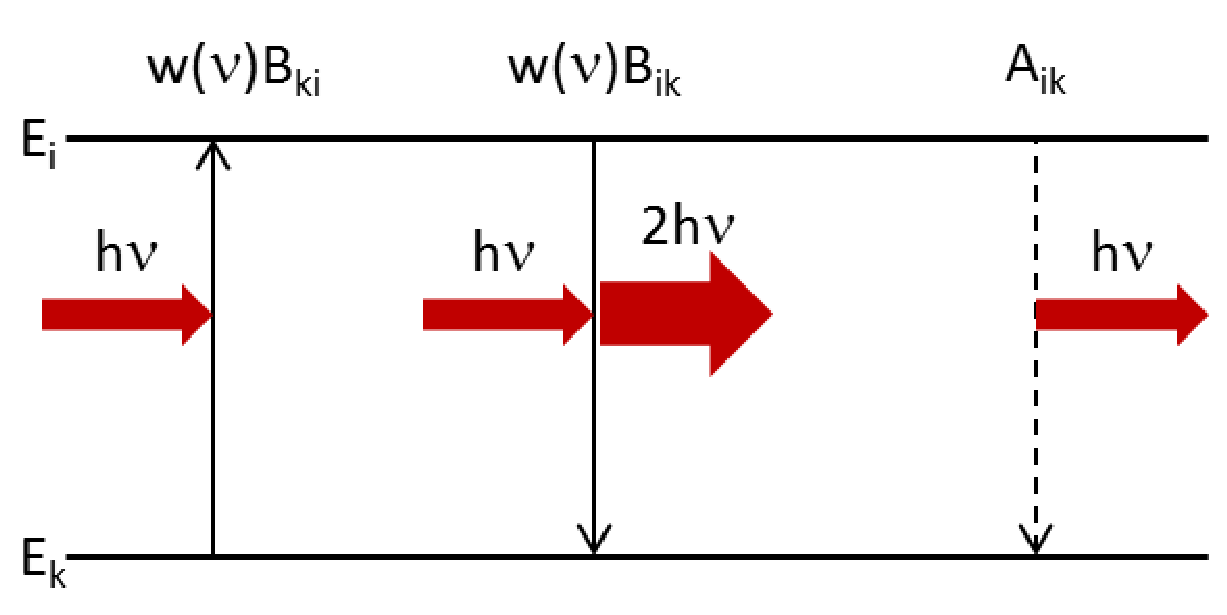
\includegraphics[width=10cm]{gfx/einstein_koeffizienten.eps}
	\caption{zwei Energieniveaus eines Atoms mit Absorption,
	induzierte Emission und spontane Emission (von links nach
	rechts)}\label{fig:einstein_koeffizienten}
\end{figure}

Im thermischen Gleichgewicht sind die Besetzungszahlen
boltzmann-verteilt \cite{demtroeder:ex3}:
\begin{equation}\label{eq:boltzmann_verteilung}
	\begin{split}
		\frac{N_i}{N_k}&=\frac{g_i}{g_k}\mathrm{e}^{-\frac{(E_i-E_k)}{kT}}\\[0.2cm]
		&=\frac{g_i}{g_k}\mathrm{e}^{-\frac{h\nu}{kT}}\,.
	\end{split}	
\end{equation}
$g_i$ und $g_k$ sind die Entartungsgrade ($2J+1$) der jeweiligen Niveaus und
sind damit eine statistische Gewichtung der Niveaus.
Kombiniert man \eqref{eq:raten_gleichung} und \eqref{eq:boltzmann_verteilung}
und löst nach $w(\nu)$ auf, findet man
\begin{equation}\label{eq:spektrale_energiedichte_1}
	w(\nu)=\frac{\nicefrac{A_{ik}}{B_{ik}}}{\left(\nicefrac{g_i}{g_k}\right)\left(\nicefrac{B_{ik}}{B_{ki}}\right)\left(\mathrm{e}^\frac{h\nu}{kT}-1\right)}\,.
\end{equation}
Führt man einen Koeffizientenvergleicht mit der spektralen
Energiedichte eines thermischen Strahlungsfeldes \cite{demtroeder:ex3}
\begin{equation}\label{eq:spektrale_energiedichte_2}
	w(\nu)=\frac{8\pi h\nu^3}{c^3}\frac{1}{\mathrm{e}^\frac{h\nu}{kT}-1}
\end{equation}
durch, findet man folgende Beziehungen der Einsteinkoeffizienten:
\begin{subequations}\label{eq:einsteinkoeff_relationen}
	\begin{equation}\label{eq:einsteinkoeff_relationen_1}
		B_{ik}=\frac{g_k}{g_i}B_{ki}
	\end{equation}
	\begin{equation}\label{eq:einsteinkoeff_relationen_2}
		A_{ik}=\frac{8\pi h\nu^3}{c^3}B_{ik}\,.
	\end{equation}
\end{subequations}
**blabla01**
\par
Im Folgenden sollen die Einsteinkoeffizienten berechnet werden.
Zur Berechnung des Koeffizienten der spontanen Emissionswahrscheinlichkeit
betrachtet man das Atom als Hertzschen Dipol, der radial isotrop abstrahlt. Die
zeitlich mittlere abgestrahlte Leistung von $N_i$ Atomen
\cite{demtroeder:ex3} ist
\begin{equation}\label{eq:abgestrahlte_leistung_01}
	\mean{P}_t = \frac{1}{3}N_i\frac{\omega_{ik}^4}{\pi\epsilon_0
	c^3}\abs{\OPv{d}_{ik}}^2
\end{equation}
mit dem bereits erwähnte Dipolmatrixelement
$\OPv{d}_{ik}=e\bra{\Psi_i}\OPv{r}\ket{\Psi_k}$. Definiert man den
Einsteinkoeffizienten der spontanen Emission $A_{ik}$ als Wahrscheinlichkeit pro
Sekunde, dass ein Atom spontan von $\ket{\Psi_i}$ in $\ket{\Psi_k}$ übergeht,
ist Gl. \eqref{eq:abgestrahlte_leistung_01} identisch mit
\begin{equation}\label{eq:abgestrahlte_leistung_02}
	\mean{P}_t=N_iA_{ik}h\nu_{ik}\,.
\end{equation}
Daraus folgt
\begin{equation}\label{eq:abgestrahlte_leistung_02}
	\boxed{
		A_{ik}=\frac{2}{3}\frac{\omega_{ik}^3}{\epsilon_0c^3h}\abs{\OPv{d}_{ik}}^2
	}\,.
\end{equation}
Um die Einsteinkoeffizienten für die Absorption und induzierte Emission
auszurechnen, setzt man mit der Absorptionswahrscheinlichkeit pro Sekunde an
(oben hergeleitete Fermis goldene Regel \eqref{eq:uebergangs_rate_total}):
\begin{equation}\label{eq:w_ki_01}
	W_{k\to i}
	= \frac{2\pi}{\hbar}\rho(E_k)\abs{\bra{\Psi_i}\OPH'\ket{\Psi_k}}^2
\end{equation}
Die Energieniveadichte lässt sich schreiben als
$\rho(E)=\pfrac{n}{E}=\frac{1}{h}\pfrac{n}{\nu}$.
Das zeitliche Mittel der spektralen Energiedichte des elektromagnetischen Feldes
ist $\mean{w(\nu)}_t=\pfrac{n}{\nu}\frac{1}{2}\epsilon_0 E^2_0$. Damit lässt
sich die Energieniveaudichte in Relation zur spektralen Energiedichte schreiben:
\begin{equation}\label{eq:energieniveaudichte_spektrale_energiedichte}
	\rho(E)=\frac{2\mean{w(\nu)}_t}{\epsilon_0 E_0^2h}\,.
\end{equation}
Setzt man Gl. \eqref{eq:energieniveaudichte_spektrale_energiedichte} in
Gl. \eqref{eq:w_ki_01} ein und schreibt das Matrixelement
zu $\bra{\Psi_i}\OPH'\ket{\Psi_k} =
\frac{1}{2}E_0\vec{\epsilon}\cdot\OPv{d}_{ki}$ um, erhält
man unter der Annahme eines isotropen Strahlungsfeldes
($\mean{\abs{\vec{\epsilon}\cdot\vr}^2} = \frac{1}{3}\abs{\vr}^2$)
\begin{equation}\label{eq:w_ki_02}
	W_{ki}
	= \frac{2\pi^2}{3h^2\epsilon_0}\abs{\OPv{d}_{ki}}^2\mean{w(\nu)}_t\,.
\end{equation}
Ein Vergleich mit Gl. \eqref{eq:einsteinkoeff_wkten_ik} liefert
\begin{equation}\label{eq:w_ki_02}
	\boxed{
		B_{ki} = \frac{2\pi^2}{3h^2\epsilon_0}\abs{\OPv{d}_{ki}}^2
	}\,.
\end{equation}
Das Ergebnis ist konsistent mit den in Gl.
\eqref{eq:einsteinkoeff_relationen} beschriebenen Relationen der
Einsteinkoeffizienten.

\subsection{Auswahlregeln}\label{subsec:auswahlregeln}
Damit ein Übergang im Rahmen der Dipolnäherung \textit{erlaubt} ist, darf das
Dipolmatrixelement nicht verschwinden:
\begin{equation}\label{eq:dipolmatrixelement}
	e\bra{\Psi_i}\OPv{r}\ket{\Psi_k}\neq0
\end{equation}
\textit{Verbotene} Übergänge können allerdings bei Betrachtung von
Matrixelementen höherer Ordnung sehr wohl erlaubt sein, sind jedoch sehr stark
unterdrückt. Welche Übergänge nun erlaubt und welche verboten sind, hängt von
der Konfiguration bzw. den Quantenzahlen der beiden Zustände ab:
\begin{equation}\label{eq:dipolmatrixelement_quantenzahlen}
	\bra{n_i,L_i,S_i,m_{L_i}, m_{S_i}}\OPv{r}\ket{n_k,L_k,S_k,m_{L_k}, m_{S_k}}
\end{equation}
Vorausgesetzt wird, dass die l-l- und s-s-Kopplungen der einzelnen Elektronen
untereinander im Atom stark gegenüber der l-s-Kopplung sind (LS-Kopplung stark).
Dies ist bei schweren Atom nicht mehr gegeben. Dort dominieren die einzelnen
l-s-Kopplungen (jj-Kopplung stark).\\
Da im Gesamtsystem die Drehimpulserhaltung
gelten muss, gilt für $\Delta L =\pm1$. Bei Absorption eines Photons wird aus dem elektromagnetischen Feld ein Photon (Boson, Spin 1) mit dem Drehimpuls vom Betrag 1 entnommen, was durch den Drehimpuls des Atoms wieder kompensiert werden muss. Analog verhält es sich bei der Emission. $\Delta L =\pm1$ kann auch mit die erforderliche unterschiedlichen Parität der Zustände begründet werden ($\OPP\ket{\psi}=(-1)^L\ket{\psi}$). Der
Ortsoperator hat ungerade Parität. Insgesamt muss sich bei der Berechnung des Matrixelements eine gerade Funktion ergeben, damit dieses von 0
verschieden ist. Dies ist nur mit unterschiedlicher Parität beider Zustände
möglich $(-1)^{L_i}\neq(-1)^{L_k}$, was für
ungerade $\Delta L$ gilt. Die Begrenzung auf $\pm1$ ist durch den Spin 1 des
Photons begründet. Die Änderung der Projektion des Drehimpulses auf die Quantisierungsachse ist mit der
Polarisation des Photons verknüpft. Bei der Absorption von zirkular
polarisiertem Licht, das sich senkrecht zur Quantisierungsachse ausbreitet, ist
der Photonen-Drehimpuls +1 für $\sigma^+$-Polarisation und -1 für
$\sigma^-$-Polarisation. Linearpolarisiertes Licht ist eine Kombination aus
$\sigma^+$- und $\sigma^-$-polarisiertem Licht. Die Projektion des Drehimpulses
ändert sich in diesem Fall nicht. Es gilt also $\Delta m_L = 0, \pm1$.
Die Spinwellenfunktion wird bei Dipolübergängen nicht beeinflusst. Daher gilt
$\Delta S=0$. Weiterhin gilt für $\vJ=\vL+\vS$ die Änderung $\Delta J=0,\pm1$.
$\Delta J=0$ rührt daher, dass die Änderung $\Delta L=\pm1$ durch die entgegengesetzte
Änderung $\Delta m_S=\mp1$ kompensiert wird, was allerdings für
$J=0\leftrightarrow0$ nicht gelten kann. Für die Kopplung an den Kernspin gilt
analoge Überlegung: $\Delta F = 0, \pm1$ außer bei $F=0\leftrightarrow0$. In
Tabelle \ref{tab:auswahlregeln} sind alle Auswahlregeln noch einmal
aufgelistet.

\begin{table}
	\begin{tabular}{p{0.17\textwidth}p{0.36\textwidth}p{0.38\textwidth}}

		\toprule
		Regel & Ursache & Einschränkungen \\
		\midrule[1px]
		\hline
		$\Delta L = \pm1$ & Parität / Gesamtdrehimpulserhaltung & in LS-Kopplung \\
		$\Delta m_L = 0, \pm1$ & Polarisation / Drehimpuls des Photons & \\
		$\Delta S = 0$ & em. Feld koppelt nicht an Spin & gilt nicht mehr für schwere
		Atome mit jj-Kopplung \\
		$\Delta m_S = 0, \pm1$ & Spinorientierung & \\
		$\Delta J = 0, \pm1$ & Spin-Drehimpuls-Kombinationen & mit Ausnahme von
		$J=0\leftrightarrow0$
		\\
		$\Delta F = 0, \pm1$ & Kernspin-J-Kombinationen & mit Ausnahme von
		$F=0\leftrightarrow0$
		\\
		\bottomrule[1px]
	\end{tabular}
	\caption{Auswahlregeln, deren Ursache und Einschränkungen}
	\label{tab:auswahlregeln}
\end{table}



\subsection{Linienprofil}\label{sec:linienprofil}
Bisher wurde noch keine Aussage über die spektrale Beschaffenheit eines
Übergangs gemacht. Diese ist aber für die Laserspektroskopie von essenzieller
Bedeutung, da sie viele Informationen über die untersuchten Atome wie z.B. die
Lebensdauern der Niveaus, Sättigungsleistungen der Laser für die Übergänge oder
die Geschwindigkeitsverteilung der Atome enthalten. Auch erfährt man durch die
Kenntnis der Linienbreite, wie hoch sich überhaupt bestimmte Übergänge auflösen
lassen und welche Lasereigenschaften dafür benötigt werden. Die
Lasereigenschaften bzw. das Laserverhalten deckt einen wesentlichen Teil
dieser Arbeit ab (siehe spätere Kapitel \ref{sec:diodenlaser}, **blabla02**).
Übergänge (hier Linien genannt) sind nicht beliebig scharf, sondern haben eine Breite, die verschiedene Ursachen hat, auf welche in diesem Abschnitt näher eingegangen werden soll. Der Großteil dieses Kapitels stützt sich auf \cite{demtroeder:laserspektroskopie}. Die spektrale Linienbreite ist durch das Frequenzintervall $\delta\omega=\omega_2-\omega_1$ zwischen den beiden
Frequenzen, bei denen die Absorptions- bzw. Emissionsintensitäten auf die Hälfte
ihres Maximums abgesunken sind, definiert (volle Halbwertsbreite, engl.: FWHM).

\subsubsection{Natürliche
Linienbreite}\label{subsubsec:natuerliche_linienbreite}
Die natürliche Linienbreite ist eine unvermeidliche, natürliche Gegebenheit.
Dies beruht darauf, dass man ein Atom (in klassischer Sichtweise) als
einen harmonischen, gedämpften Oszillator ansehen kann, dessen Frequenzspektrum
nicht diskret ist. Die Lösung der Bewegungsgleichung eines klassischen
Oszillators
\begin{equation}\label{eq:klassischer_oszillator_bewegungsgleichung}
	\ddot x+\gamma\dot x+\omega_0^2x=0
\end{equation}
ist
\begin{equation}\label{eq:klassischer_oszillator_loesung}
	x(t)=x_0\mathrm{e}^{-\nicefrac{\gamma t}{2}}\left[\cos(\omega
	t)+\frac{\gamma}{2\omega}\sin{(\omega t)}\right]\quad
	\text{mit}\quad \omega=\sqrt{\omega_0^2-\frac{\gamma^2}{4}}\,.
\end{equation}
Um das Frequenzspektrum zu erhalten, führt man eine Fouriertransformation durch
($x(t)\to A(\omega)$). Unter Berücksichtigung, dass man sich in nahresonanter
Umgebung befindet ($(\omega-\omega_0)^2\ll\omega_0^2$), folgt die auf die
Gesamtintensität $I_0$ normierte spektrale Intensitätsverteilung als sog.
\textit{Lorentz-Profil}
\begin{equation}\label{eq:klassischer_oszillator}
	\begin{split}
		I(\omega) &=A(\omega)A^*(\omega)\\
		&=
		I_0\frac{\nicefrac{\gamma}{2\pi}}{(\omega-\omega_0)^2+(\nicefrac{\gamma}{2})^2}\,.
	\end{split}
\end{equation}
Hierbei ist $\delta\omega_n=\gamma$ die natürliche Linienbreite. Weiterhin lässt
sich hier auch ein Zusammenhang zwischen der Linienbreite und der Lebensdauer
eines Zustandes herleiten. Multipliziert man die Bewegungsgleichung
\eqref{eq:klassischer_oszillator_bewegungsgleichung} mit $m\dot x$ und führt
eine Zeitableitung durch, findet man
\begin{equation}\label{eq:klassischer_oszillator_lebensdauer_01}
	\fracd{}{t}\left[\frac{m}{2}\dot
	x^2+\frac{m}{2}\omega_0^2x^2\right]=-\gamma m\dot x^2=\fracd{W}{t}=P(t)\,.
\end{equation}
wobei $W$ die Gesamtenergie und $P(t)$ die momentan abgestrahlte Leistung des
Atoms ist. Nach Einsetzen von \eqref{eq:klassischer_oszillator_loesung} in
\eqref{eq:klassischer_oszillator_lebensdauer_01} und zeitliche Mittlung findet
man
\begin{equation}\label{eq:klassischer_oszillator_lebensdauer_01}
	\mean{P(t)}_t=-\frac{1}{2}\gamma mx_0^2\omega_0^2\mathrm{e}^{-\gamma
	t}\propto\mathrm{e}^{-\gamma
	t}\,.
\end{equation}
Dies bedeutet, dass die Leistungsabnahme nach $\tau=\nicefrac{1}{\gamma}$ auf
$\nicefrac{1}{\mathrm{e}}$ des Anfangswertes abgefallen ist. Folglich ist die
Linienbreite eines spontanen Zerfalls von einem Niveau $E_i$ in den Grundzustand
$\delta\omega_i=\nicefrac{1}{\tau_i}$. Zu diesem Ergebnis kommt man auch über
die Heisenbergsche Unschärferelation bei scharf bestimmtem $\tau$:
\begin{equation}\label{eq:unschaerferelation}
	\begin{split}
		\Delta E\cdot\Delta t &\geq2\pi\hbar\\
		&\Leftrightarrow\\
		\hbar\,\delta\omega\cdot2\pi\tau &\geq2\pi\hbar\\
		&\Leftrightarrow\\
		\delta\omega &\geq\frac{1}{\tau}\,.
	\end{split}
\end{equation}
Die Linienbreite eines Übergangs zwischen
zwei angeregten Niveaus $E_i$ und $E_k$ ergibt sich aus den Lebensdauern beider Niveaus mit
\begin{equation}\label{eq:natuerliche_linienbreite_lebensdauern}
	\delta\omega_{i\leftrightarrow
	k}=\frac{1}{\tau_i}+\frac{1}{\tau_k}\,.
\end{equation}

\subsubsection{Sättigungsverbreiterung}\label{subsubsec:saettigungsverbreiterung}
Die Sättigunugsverbreiterung der Linie tritt erst durch Einstrahlen von
Laserlicht in Erscheinung. Sie ist gerade bei hohen Laserleistungen von
Bedeutung. Sehr elegant lässt sich die Sättigungsverbreiterung über den
\textit{Dichtematrix-Formalismus} herleiten.\\
Im Experiment sind die Atome aufgrund der spontanen Emission statistisch
verteilt und somit dephasiert. Es liegt kein \textit{reiner Zustand}\footnote{Reiner Zustand: Es
besteht eine kohärente Überlagerung der Zustände:
$\ket{\Psi}=\frac{1}{\sqrt{2}}\left[\alpha(t)\mathrm{e}^{\mathrm{i}\phi}\keta+\beta(t)\ketb\right]$,
wobei die Phase $\phi$ immer konstant bleibt.} mehr vor, sondern ein
\textit{statistisches Gemisch}. Die Phase zwischen den Zuständen ist
für jedes Atom individuell im Intervall $[0,2\pi)$ verteilt. Somit ist eine einfach Behandlung mit der Schrödingergleichung nicht mehr
möglich. Der Dichtematrix-Formalismus berücksichtigt diese Tatsache
allerdings.\\
Dazu betrachtet mach sich die Dichtematrix:
\begin{equation}\label{eq:dichtematrix}
	\OP{\rho}
	=
	\begin{pmatrix}
		\rho_{11} & \rho_{12}\\
		\rho_{21} & \rho_{22}
	\end{pmatrix}
	=
	\begin{pmatrix}
		c_1c_1^* & c_1c_2^*\\
		c_2c_1^* & c_2c_2^*
	\end{pmatrix}\,.
\end{equation}
$\rho_{11}$ bzw. $\rho_{22}$ sind die Besetzungswahrscheinlichkeiten von
$\ket{1}$ bzw. $\ket{2}$. $\rho_{12}$ und $\rho_{21}$ sind die
Kohärenzen beider Zustände, wobei $\rho_{12}=\rho_{21}^*$ ist. $c_i$ bzw.
$c_i^*$ sind wiederum die Zeitentwicklungskoeffizienten der Zustände $\ket{i}$.
Die Bewegungsgleichungen dieser Koeffizienten erlangt man aus dem
nicht-störungstheoretischen Ansatz eines 2-Niveau-Systems, welcher wie folgt
aussieht:
\begin{subequations}\label{eq:2-niveau-system_ansatz}
	\begin{equation}\label{eq:2-niveau-system_ansatz_hamilton}
		\begin{split}
			\OPH &=\OPH_0-\vd\cdot\vE(t)\\
			\text{mit}\quad
			\vE(t) &=\vec{\epsilon}E_0\cos{(\omega t)}\\
			\text{und}\quad
			\OPH_0 &=\hbar\omega_1\ket{1}\bra{1}+\hbar\omega_2\ket{2}\bra{2}
		\end{split}
	\end{equation}
	\begin{equation}\label{eq2-niveau-system_ansatz_zustand}
		\ket{\Psi}=c_1(t)\mathrm{e}^{-\mathrm{i}\omega_1
		t}\ket{1}+c_2(t)\mathrm{e}^{-\mathrm{i}\omega_2 t}\ket{2}\,.
	\end{equation}	
\end{subequations}
Gleichung \ref{eq:2-niveau-system_ansatz_hamilton} beschreibt den
Hamilton-Operator, Gleichung \ref{eq2-niveau-system_ansatz_zustand} beschreibt
den Zustand eines 2-Niveau-Systems. Nach Einsetzen in die Schrödingergleichung
und etwas längerer Rechnung findet man
\begin{subequations}\label{eq:2-niveau-system_koeffizienten}
	\begin{equation}\label{eq:2-niveau-system_c1}
		\dot c_1(t)=\frac{\mathrm{i}\Omega_0}{2}\mathrm{e}^{\mathrm{i}\delta t}c_2(t)
	\end{equation}
	\begin{equation}\label{eq2-niveau-system_ansatz_c2}
		\dot c_2(t)=\frac{\mathrm{i}\Omega_0}{2}\mathrm{e}^{\mathrm{i}\delta
		t}c_1(t)\,,
	\end{equation}	
\end{subequations}
wobei $\delta$ die Verstimmungsfrequenz zwischen Lichtfeld und atomarem Übergang
ist ($\delta=\omega-\omega_{21}$). $\Omega_0=\nicefrac{dE_0}{\hbar}$ ist die
sog. \textit{Rabifrequenz}\footnote{Die Rabifrequenz
ist die Frequenz mit der das 2-Niveau-System zwischen Grundzustand und
angeregtem Zustand oszilliert, sofern kontinuierlich resonantes Licht
eingestrahlt wird.}, welche aber im Folgenden von keinem Interesse ist.
Betrachtet man die Zeitentwicklung der Dichtematrixelemente
\begin{equation}\label{eq:dichtematrix_zeitentwicklung}
	\fracd{}{t}\OP{\rho}
	=
	\begin{pmatrix}
		\dot c_1c_1^*+c_1\dot c_1^* & \dot c_1c_2^*+c_1\dot c_2^*\\
		\dot c_2c_1^*+c_2\dot c_1^* & \dot c_2c_2^*+c_2\dot c_2^*
	\end{pmatrix}
\end{equation}
und setzt nun Gln. \ref{eq:2-niveau-system_koeffizienten} in Gl.
\ref{eq:dichtematrix_zeitentwicklung} ein ergeben sich die sog.
\textit{optischen Blochgleichungen} (OBE's):
\begin{subequations}\label{eq:blochgleichungen_01}
	\begin{equation}\label{eq:blochgleichungen_11}
		\fracd{}{t}\rho_{11}=\gamma\rho_{22}+\mathrm{i}\frac{\Omega_0}{2}(\tilde\rho_{21}-\tilde\rho_{12})
	\end{equation}
	\begin{equation}\label{eq:blochgleichungen_22}
		\fracd{}{t}\rho_{22}=-\gamma\rho_{22}+\mathrm{i}\frac{\Omega_0}{2}(\tilde\rho_{12}-\tilde\rho_{21})
	\end{equation}
	\begin{equation}\label{eq:blochgleichungen_12}
		\fracd{}{t}\tilde\rho_{12}=-\left(\frac{\gamma}{2}+\mathrm{i}\delta\right)\tilde\rho_{12}+\mathrm{i}\frac{\Omega_0}{2}(\rho_{22}-\rho_{11})
	\end{equation}
	\begin{equation}\label{eq:blochgleichungen_21}
		\fracd{}{t}\tilde\rho_{21}=-\left(\frac{\gamma}{2}+\mathrm{i}\delta\right)\tilde\rho_{21}+\mathrm{i}\frac{\Omega_0}{2}(\rho_{11}-\rho_{22})\,.
	\end{equation}	
\end{subequations}
Hierbei wurde direkt schon die spontane Emissionsrate $\gamma$ von Niveau
$\ket{2}$ zu Niveau $\ket{1}$ eingepflegt.
$\tilde\rho_{12}=\mathrm{e}^{-\mathrm{i}\delta t}\rho_{12}$ und $\tilde\rho_{21}=\mathrm{e}^{\mathrm{i}\delta
t}\rho_{21}$ bedeutet, dass $\rho_{ij}$ ($i\neq j$) in ein rotierendes
Bezugssystem mit Frequenz $\delta$ transformiert worden sind. Da für die
Kohärenzen $\rho_{12}=\rho_{21}^*$ gilt, reduzieren sich die OBE's zu zwei
unabhängigen Gleichungen
\begin{subequations}\label{eq:blochgleichungen_01}
	\begin{equation}\label{eq:blochgleichungen_21}
		\fracd{}{t}\tilde\rho_{21}=-\left(\frac{\gamma}{2}-\mathrm{i}\delta\right)\tilde\rho_{21}-\frac{\mathrm{i}w\Omega_0}{2}
	\end{equation}
	\begin{equation}\label{eq:blochgleichungen_w}
		\fracd{}{t}w=-\gamma(w+1)-\mathrm{i}\Omega_0(\tilde\rho_{21}-\tilde\rho_{12})
	\end{equation}	
\end{subequations}
mit der \textit{Besetzungsinversion} $w=\rho_{22}-\rho_{11}$. Sie gibt an, wie
stark die Besetzung im Zustand $\ket{2}$ gegenüber der im Zustand $\ket{1}$ ist.
Für lange Zeiten stellt sich eine Gleichgewichtslösung ein. Dies ist mit der Bedingung gegeben, dass sich
die Besetzungsinversion und die Kohärenzen nicht mehr ändern:
\begin{equation}\label{eq:blochgleichungen_gleichgewicht}
	\begin{split}
		\fracd{}{t}\tilde\rho_{21} &=\fracd{}{t}w=0\\
		&\Leftrightarrow\\
		w &=-\frac{1}{1+S}\\
		\text{und}\quad
		\tilde\rho{21}
		&=\frac{\mathrm{i}\Omega_0}{2(\nicefrac{\gamma}{2}-\mathrm{i}\delta)(1+S)}\,.
	\end{split}
\end{equation}
Hier wurde der \textit{Sättigungsparameter}
\begin{equation}\label{eq:saettigungsparameter}
	S=\frac{S_0}{1+\nicefrac{4\delta^2}{\gamma^2}}
\end{equation}
mit dem \textit{resonanten Sättigungsparameter}
\begin{equation}\label{eq:saettigungsparameter_0}
	S_0=\frac{2\Omega_0^2}{\gamma^2}
\end{equation}
eingeführt. Für die Population des angeregten Zustandes erhält man mit
$\rho_{11}+\rho_{22}=1$
\begin{equation}\label{eq:besetzung_22}
	\rho_{22}=\frac{1}{2}(1+w)=\frac{S}{2(1+S)}=\frac{\nicefrac{S_0}{2}}{1+S_0+\nicefrac{4\delta^2}{\gamma^2}}\,.
\end{equation}
Hieraus ergibt sich die Photonenstreurate
\begin{equation}\label{eq:photonenstreurate_01}
	\Gamma_{ph}=\gamma\rho_{22}=\frac{\gamma}{2}\frac{S_0}{1+S_0+\nicefrac{4\delta^2}{\gamma^2}}\,,
\end{equation}
die im Gleichgewicht gleich der Absorptionsrate ist.
Nach einer Umformung
\begin{equation}\label{eq:photonenstreurate_01}
	\Gamma_{ph}=\left(\frac{S_0}{1+S_0}\right)\left(\frac{\nicefrac{\gamma}{2}}{1+\nicefrac{4\delta^2}{\gamma'^2}}\right)
	\quad\text{mit}\quad
	\gamma'=\gamma\sqrt{1+S_0}
\end{equation}
sieht man etwas sehr interessantes: 

\section{Resonanz-Ionisations-Spektroskopie}\label{sec:ris}

\section{Diodenlaser in der RIS}\label{sec:diodenlaser}
%\cite{chow:semiconductor-laser}
\section{Experimenteller Aufbau}
In diesem Kapitel soll der experimentelle Aufbau des gesamten Lasersystems und
dessen Kopplung an die Vakuumapperatur und den Quadrupol beschrieben werden.
Zunächst wird ein Überblick über das gesamte System gegeben (Abschn.
\ref{sec:gesamtaufbau}). Abschnitt \ref{sec:lasersystem} beschriebt den gesamten
optischen Aufbau inklusive Laserstabilisierung. Die Weiterverarbeitung der
Laserinformation und die Stabilisierung sollen in Abschn.
\ref{sec:elektronik_laserkontrolle} genauer betrachtet werden. Da
hard- und softwareseitige Implementierung der Laserkontrolle eng miteinander verknüpft
sind, kommt es zu Überschneidungen mit Kap. \ref{kap:software}, in dem die
softwareseitige Realisierung genau erklärt wird. In Abschn.
\ref{sec:vakuum-aparatur_qms} wird kurz speziell auf die verwendete
Vakuumaparatur und dem daran gekoppelten Quadrupolmassenseperator eingegangen.

\section{Gesamtaufbau}\label{sec:gesamtaufbau}
\begin{figure}[h]
 	\centering
 	\fbox{\parbox{\dimexpr \linewidth - 2\fboxrule - 2\fboxsep}{
 	\centering
	    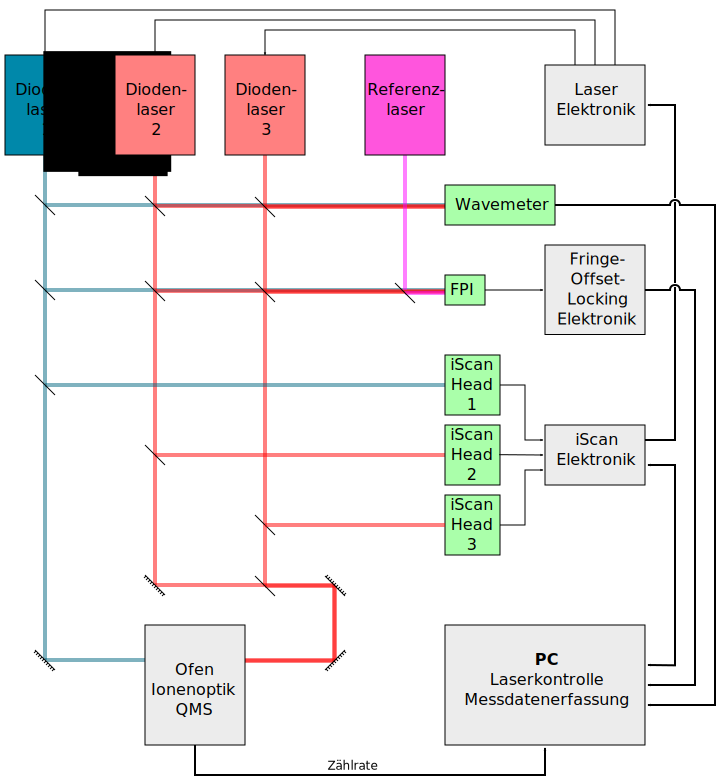
\includegraphics[width=\textwidth-2cm]{gfx/experimenteller_aufbau_gesamt}
	}}
	\caption[Gesamter experimenteller Aufbau, schematisch]{Gesamter experimenteller
	Aufbau des Systems (schematisch).}\label{fig:experimenteller_aufbau_gesamt}
\end{figure}
Abbildung \ref{fig:experimenteller_aufbau_gesamt} zeigt schematisch den gesamten
Aufbau des Systems. Das zur resonanten Anregung nötige Licht wird mit drei
Diodenlaser erzeugt. Der größte Teil des Lichts wird möglichst
direkt in die Vakuumaparatur, die aus einem Ofen für das Ausheizen der Atome,
einer Ionenoptik für die Kontrolle der erzeugten Ionen und einem
Quadrupolmassenseperator (QMS) zur Massenselktion der Ionen besteht, geführt.
Die Einstrahlung der Laser erfolgt aus den in Abschn. \ref{sec:linienprofil}
erleuterten Gründen transversal zum aus dem Ofen austretenden kollimierten Atomstrahl.
Abgriffe der Hauptstrahlen führen das Laserlicht eines jeden Lasers in ein
Wavemeter, das die Absolutwellenlängen liefert und an einen PC weiterleitet.
Zwei jeweils weitere Abgriffe führen die Strahlen in die Optiken iScan Heads und FPI der zwei verwendeten
Laserstabilisierungen. Die dort erzeugten Signale werden an die jeweilige Elektronik
weitergeleitet. Die Elektronik eines iScan Heads ist die iScans control units, die direkt an die Elektronik des entsprechenden Laser
angeschlossen ist und sowohl die Spannung des Laserpiezos als auch den Strom
der Laserdiode moduliert. Die Elektronik des Fringe-Offset-Locking bereitet die
analogen Signale des FPIs digital auf und leitet sie weiter an den PC, der
gleichzeitig mit den iScan control units bidirektional verbunden ist und die
Regelung der iScan-Sollwerte übernimmt. Weiterhin kann mit dem PC die Zählrate
der Ionen, die einzeln durch ein hinter dem QMS angebrachten Channeltron
detektiert werden, aufgenommen werden. Die Steuerung des Massenseperators
bezüglich der Einstellung bzw. des Scans bestimmter Massen durch den PC wurde im
Rahmen dieser Arbeit noch nicht realisiert, soll aber nachträglich implementiert
werden. Alternativ wird hierfür bis zum Abschluss dieser Arbeit noch ein PC des
Vorgängersystems verwendet.

\section{Lasersystem}\label{sec:lasersystem}
\begin{figure}[h]
 	\centering
 	\fbox{\parbox{\dimexpr \linewidth - 2\fboxrule - 2\fboxsep}{
 	\centering
	    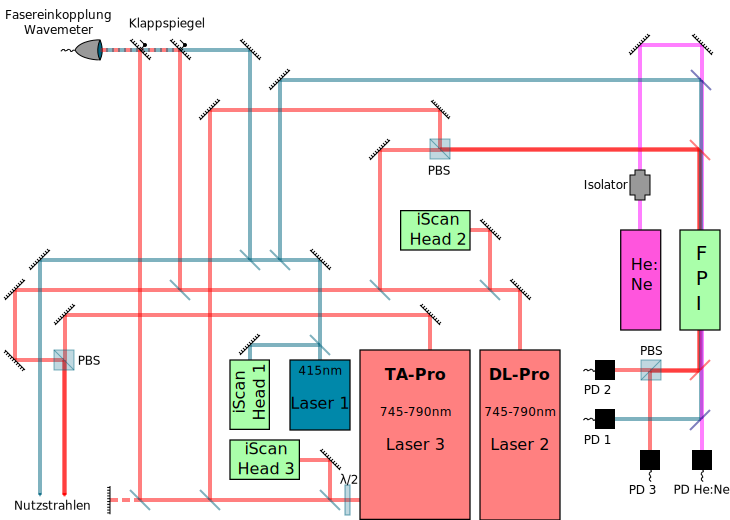
\includegraphics[width=\textwidth-2cm]{gfx/experimenteller_aufbau_lasersystem}
	    }}
	\caption[Experimenteller Aufbau des Lasersystems, schematisch]{Experimenteller
	Aufbau des Lasersystems
	(schematisch).}\label{fig:experimenteller_aufbau_lasersystem}
\end{figure}
Ein detaillierter Aufbau des Lasersystems wird schematisch durch Abb.
\ref{fig:experimenteller_aufbau_lasersystem} veranschaulicht und ist als
Fotografie in Abb. \ref{fig:experimenteller_aufbau_lasersystem_foto} noch einmal
zu sehen.\par
Das Laserlicht für den ersten Anregungsschritt wird in einem nach dem
Littrow-Design gebauten Diodenlaser erzeugt. Eingebaut ist eine blaue
$415\,$nm-Laserdiode mit einem Verstärkungsprofil von $\pm1\,$nm bei
zugeschalteten externen Resonator. Der modensprungfreie Verstimmungsbereich ist
mit $15\,$GHz spezifiziert. In manchen Moden wurden allerdings auch Verstimmungsbereiche
von bis zu $20\,$GHz erreicht. Das Laserlicht des zweiten und dritten
Anregungsschritts wird mit zwei kommerziellen, ebenfalls im Littrow-Design
gebauten, roten Diodenlasern der Firma Toptica erzeugt.
Beide Dioden haben ein spezifiziertes Verstärkungsprofil von
$745\,$nm bis $790\,$nm und einen modensprungfreien Verstimmungsbereich von bis
zu $30\,$GHz, was bestätigt wurde. Weiterhin kann das Laserlicht der Diode für
den dritten Anregungsschritt mit einem Trapezverstärker wahlweise bis auf eine
Leistung von $1,5\,$W verstärkt werden. Neben dem leistungsstarken Nutzstrahl
gibt es noch die Möglichkeit, einen Teil des zum Injection-Seeding verwendeten
Masterlaserstrahl abzugreifen (links unten am TA-Pro in Abb.
\ref{fig:experimenteller_aufbau_lasersystem}). Für den ersten bzw.
zweiten Anregungsschritt können ca. $7\,$mW bzw. ca. $60\,$mW bei Diodenströmen von ca. $35\,$mA bzw. ca.
$120\,$mA erreicht werden, was für die Untersuchung von Uran-Isotopen
ausreichend ist. Die Sättigungsleistungen sind im ersten Schritt $<1\,$mW, im
zweiten Schritt wenige mW und im dritten Schritt wenige $100\,$mW. Tabelle \ref{tab:laser_spezifikationen} listet noch einmal alle
Laser-Spezifikationen auf.
***blabla*Referenz zu Lasermanuals / Diodenmanuals*blabla***\par
\begin{table}
	%Summe der Breiten muss 0.91 mal \textwidth sein.
	\begin{tabular}{p{0.23\textwidth}|p{0.24\textwidth}p{0.24\textwidth}p{0.24\textwidth}}
		\toprule
		& Laser 1 & Laser 2 & Laser 3\\
		\midrule[1px]
		\hline
		Bezeichnung & Eigenbau & DL-Pro & TA-Pro\\
		Wellenlänge & $415\pm1\,$nm & $745\,$-$790\,$nm & $745\,$-$790\,$nm\\
		max. Leistung & $7\,$mW & $60\,$mW & $1,5\,$W\\
		nötige Leistung & $<1\,$mW & $xx\,$mW & $xxx\,$mW\\
		Externer Resonator & Littrow & Littrow & Littrow\\
		\bottomrule[1px]
	\end{tabular}
	\caption[Spezifikationen der verwendeten Diodenlaser]{Spezifikationen der
	verwendeten Diodenlaser}
	\label{tab:laser_spezifikationen}
\end{table}
Die Teilstrahlen für die Stabilisierung der iScans werden auf Grund der in
\ref{subsec:iScan} erklärten Empfindlichkeit auf räumliche Drifts möglichst
direkt in die iScan Heads geführt, damit die Hebelwirkung bei Drifts möglichst
gering ist. Für das iScan für Laser 3 muss die Polarisation mit einem
$\nicefrac{\lambda}{2}$-Plättchen gedreht werden.\par Die Abgriffe für das Wavemeter des Typs ***blabla*Typ*blabla*** von der Firma
High Finesse müssen mit Klappspiegeln einzeln ausgewählt werden, da immer nur das
Licht eines Lasers im Wavemeter analysiert werden kann. Die Genauigkeit des
Wavemeters von $30\,$MHz hat ***blabla*Referenz zu Wavemeter-Manual*blabla***,
würde es zur Frequenzstabilisierung nicht genügen, ist aber für das Finden von Resonanzen und wie schon erwähnt zum Berechnen der Relativfrequenzen nach Gl. \eqref{eq:FPI_frequenzdrift_03}
ausreichend.\par
Für das Fringe-Offset-Locking muss das Licht aller drei zu stabilisierenden
Laser vor dem FPI zusammengeführt und danach wieder getrennt werden. Da die
Wellenlängen von Laser 2 und 3 sehr nahe beieinander liegen, muss das Licht
dieser Laser mit Polarisationsstrahlteiler zusammengeführt und getrennt werden.
Dabei ist zu beachten, dass die Verluste durch die jeweils falsche Polarisation
der Laser möglichst gering ist, was durch optionales Drehen der
Polarisation mit $\nicefrac{\lambda}{2}$-Plättchen möglich ist. Die Überlagerung
mit dem blauen Licht des ersten Lasers und dem He:Ne-Laser kann mit
dichroitischen Spiegeln realisiert werden. Diese sind dafür ausgelegt bestimmte
Wellenlängenbereiche zu reflektieren, während andere bestimmte Bereiche
transmittiert werden. Die Trennung der Strahlen erfolgt nach dem selben
Prinzip. Hinter dem gerampten FPI wird das Fringepattern aller vier Laser
getrennt mit Photodioden aufgenommen. Das FPI hat nach Angaben aus dem Jahre 199x einen
freien Spektralbereich von $298,xx\,$MHz. Im nah-infraroten Bereich hat es die
größte Finesse, wohingegen im blauen Bereich die Finesse sehr schlecht ist.
Das Fringe-Offset-Locking ist damit zwar noch möglich, es wird allerdings
angestrebt, ein anderes Interferomter zu verwenden. Dieses wird momentan
noch in dem parallel laufenden alten System verwendet, das während dem
Entstehen dieser Arbeit noch als Referenzsystem eingesetzt und in
\ref{sec:altes_lasersystem} kurz beschrieben wird.\par
Die Hauptstrahlen werden an ein Pereskop geführt, über das das Licht in einen
anderen Raum an die Vakuum-Aparatur transportiert wird, wobei das Licht von
Laser 2 und 3 wieder durch Polarisationstrennung überlagert ist. Der
Strahltransport über das Pereskop ist Teil einer Vorablösung, da auf dem
Lasertisch der Vakuum-Aparatur das alte Lasersystem aufgebaut ist.\par
Der He:Ne-Laser ist gegen Rückreflexe aus dem FPI durch einen optischen Isolator
geschützt. Ebenso hat der zweite Laser vor dem Masterlaserabgriff und nach dem
Trapezverstärker einen Isolator. Laser 1 und 2 haben momentan noch keinen
Isolator. Es soll jedoch in Zukunft jeweil ein Isolator zwischengeschaltet
werden.

\section{Elektronik der Laserkontrolle}\label{sec:elektronik_laserkontrolle} In
diesem Abschnitt wird die Verarbeitung der Signale zur Laserkontrolle schematisch erklärt. Für
Schaltpläne und interne elektronische Abläufe verschiedener Komponenten sei auf
den Anhang verwiesen. Abbildung \ref{fig:experimenteller_aufbau_elektronik_laserkontrolle} zeigt den
schematischen Aufbau der Elektronik für die Laserkontrolle.\par
\begin{figure}[h]
 	\centering
 	\fbox{\parbox{\dimexpr \linewidth - 2\fboxrule - 2\fboxsep}{
 	\centering
	    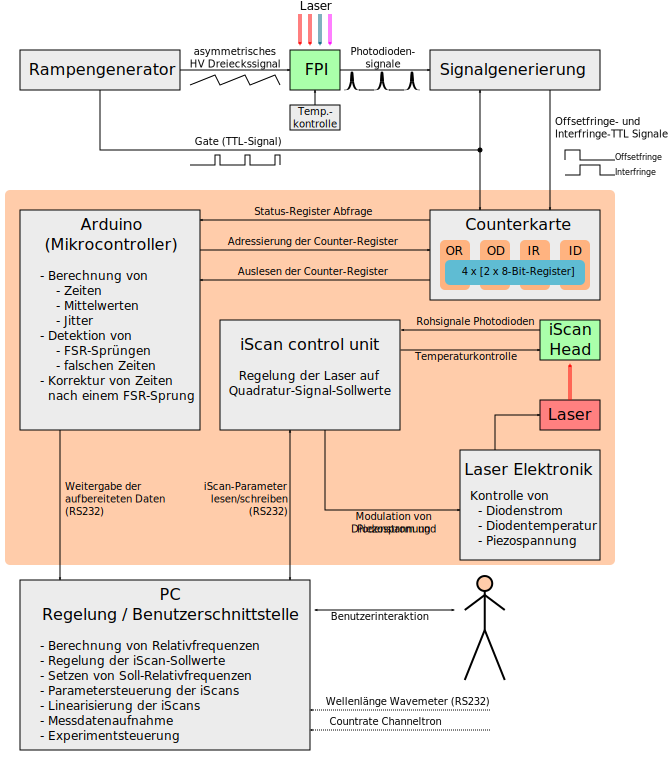
\includegraphics[width=\textwidth-2cm]{gfx/experimenteller_aufbau_elektronik_laserkontrolle}
	    }}
	\caption[Experimenteller Aufbau der Laserkontollelektronik,
	schematisch]{Experimenteller Aufbau der Elektronik der Laserkontrolle
	(schematisch).}\label{fig:experimenteller_aufbau_elektronik_laserkontrolle}
\end{figure}
Das FPI wird durch einen Rampengenerator in seiner Länge linear durchgefahren.
Dazu wird ein asymetrisches Dreieckssignal mit ca. $60\,$Hz erzeugt, welches die wie in Abb.
\ref{fig:FPI_signal-zeitverlauf}(b) gezeigte Fringepattern für jeden Laser
an den Photodioden hinter dem FPI erzeugt. Außerdem gibt der Rampengenerator
ein TTL-Signal aus, des bei fallender Spannungsflanke HIGH und bei
steigender Spannungsflanke LOW ist. Die fallende bzw. steigende Flanke dieses
\textit{Gates} signalisiert also den Start bzw. das Ende der Spannungsrampe
und wird als Triggersignal verwendet. Die Photodiodensignale und das
Gate werden an einen Signalgenerator weitergegeben, welcher über Ableiten der
Fringesignale die wie in \ref{fig:FPI_signal-zeitverlauf}(d,e) gezeigten TTL-Pulse erzeugt.
Wie dies genau geschieht wird in Anh. \ref{anh:kap:signalgenerierung}
beschrieben. Es ist weiterhin möglich, eine \textit{Delay} in der Detektion des
ersten Fringes einzustellen, damit Nichtlinearitäten zu Beginn der Rampe
ignoriert werden.\par
Der im Folgenden beschriebene Ablauf ist für jeden zu stabilisierenden Laser
gleich. Daher wird dieser Teil exemplarisch für einen Laser und den
Referenzlaser beschrieben. Die durch den Offsetfringe und Interfringe erzeugten
TTL-Pulse des sowohl zu stabilisierenden Lasers als auch des Referenzlasers,
sowie das Gate werden an eine Counterkarte weitergeleitet. Diese besteht aus
vier 16-Bit-Countern und einem Taktgeber mit einstellbarer Taktrate ($1,25\,$,
$2,5\,$, $5\,$ und $10\,$MHz), wodurch unterschiedliche Zeitauflösungen möglich
sind ($0,8\,$, $0,4\,$, $0,2\,$ und $0,1\,$\textmu s).
Wird das Gate auf LOW gesetzt (Beginn der steigenden Spannungsflanke), werden
alle Counter freigeschaltet. Wenn die durch
das Delay etwas verzögerten TTL-Signale der Offsetfringes auf HIGH gesetzt werden, beginnen die
entsprechenden Counter der Offsetfringes (OR und OD) zu zählen. Beim eintreten
der Interfringes werden die Counter gestoppt und die Counter für die
Interfringezeiten gestartet (IR und ID). Am Ende der steigenden Spannungsflanke
wird das Gate auf HIGH gesetzt und die Counter werden gesperrt. Beim Stoppen eines
jeden Counters liegen die Counterwerte in jeweils 2x8-Bit-Registern
(\textit{Upper Byte} und \textit{Lower Byte}) vor und es wird jeweils ein
\textit{Ready-Bit} gesetzt, welches Abrufbereitschaft der entsprechenden
Counterwerte signalisiert.\par
Die Ready-Bits sind über ein \textit{Statusregister} auslesbar. Die Adressierung
der einzelnen Counterregister wird über einen \textit{Adressbus} mit vier Bits
gesteuert, dessen Kodierung in Tab. \ref{tab:adressbus_kodierung} aufgeschlüsselt ist.
\begin{table}
	%Summe der Breiten muss 0.91 mal \textwidth sein.
	\begin{tabular}{p{0.1\textwidth}p{0.1\textwidth}p{0.1\textwidth}p{0.1\textwidth}|p{0.51\textwidth}}
		\toprule
		Enable & Addr. 1 & Addr. 2 & Addr. 3 & Wirkung\\
		\midrule[1px]
		\hline
		L & - & - & - & Adressierung deaktiviert\\
		H & L & L & L & Lower Byte Offsetfringe Referenzlaser\\
		H & L & L & H & Upper Byte Offsetfringe Referenzlaser\\
		H & L & H & L & Lower Byte Interfringe Referenzlaser\\
		H & L & H & H & Upper Byte Interfringe Referenzlaser\\
		H & H & L & L & Lower Byte Offsetfringe Diodenlaser\\
		H & H & L & H & Upper Byte Offsetfringe Diodenlaser\\
		H & H & H & L & Lower Byte Interfringe Diodenlaser\\
		H & H & H & H & Upper Byte Interfringe Diodenlaser\\
		\bottomrule[1px]
	\end{tabular}
	\caption[Adressierung Counterregister]{Aufschlüsselung der Adressierung der
	Counterregister}
	\label{tab:adressbus_kodierung}
\end{table}
Dabei sind \textit{Addr. 1} bis \textit{3} die Adressleitungen. Über
\textit{Enable} kann die Adressierung aktiviert und deaktiviert werden. Sehr
wichtig hierbei ist, dass einem Adressierungswechsel auf ein anderes
Counterregister die Adressierung immer deaktiviert werden muss. Andernfalls kann
es zur Zerstörung der Counter kommen.\par
Die Auslese und Weiterverarbeitung der Werte muss nun bis spätestens zur
nächsten steigenden Spannungsrampe abgeschlossen sein, damit die neuen
Rampensignale abgearbeitet werden können und es zu keinen Datenverlusten kommt.
Da bei einem PC mit Windows-Betriebssystem die Prozessverwaltung auf Grund von
unvorhersehbaren Interupts nie deterministisch ist, ist es sehr unsicher die
Daten direkt mit einem PC zu verarbeiten. Daher werden die Daten zunächst von
einem Mikrocontroller aufbereitet und anschließend an einen PC gesendet. Als
Mikrocontroller eignet sich dafür hervorragend die Entwicklungsplattform
\textit{Arduino$^\text{\textregistered}$}\footnote{http://www.arduino.cc}. Diese
wird verwendet, da sich das Projekt auch nach Abschluss dieser Arbeit noch in
der Entwicklungsphase befindet und der Arduino eine unkomplizierte Handhabung
und Programmierung bietet, was für Entwicklungszwecke gegenüber einem einfachen
Mikrocontroller-Chip sehr viel vorteilhafter ist. Der hier eingesetzte
\textit{Arduino Mega 2560} bietet 54 digitale Ein- und Ausgänge, hat eine
Taktrate von $16\,$MHz Flashspeicher von $256\,$kb für den binären Programmcode.

\section{Ergebnisse und Diskussion}
\include{ergebnisse_und_diskussion.tex}
\section{Zusammenfassung und Ausblick}
Im Rahmen dieser Arbeit wurde eine Frequenzstabilisierung für das
umfangreiche Diodenlasersystem zur HR-RIMS an Uranisotopen entwickelt und
getestet. Dabei wurde auf die bewährte Stabilisierungstechnik \textit{Fringe-Offset-Locking} zurückgegriffen, welche
durch eine weitere kommerzielle interferometrische Technik (\textit{iScan})
ergänzt wurde, um einen Zugewinn an Geschwindigkeit und Sicherheit der Stabilisierung bzw. der
Frequenzverstimmungen zu erhalten.
Ein Teil der digitalen Datenverarbeitung der Stabilisierung wurde dabei auf
Mikrocontroller ausgelagert, um das deterministische Verhalten des Systems zu steigern. Zur
Experimentsteuerung, Laserkontrolle und Datenaufnahme wurde ein
\textit{Labview}-Programm entwickelt, mit dem Messungen
automatisch und ohne großen Aufwand durchgeführt werden können.\par
Damit die Frequenzkontrolle korrekte Werte liefert und die Laser auf die
richtigen Frequenzen stabilisiert werden können, musste der freie
Spektralbereich des Fabry-Perot-Interferometers neu vermessen werden. Dieser
konnte mit einer Genauigkeit von $8,7\cdot10^{-6}$ auf $(298,0856\pm0,0026)$MHz
bestimmt werden.\par
Weiterhin wurde die Frequenzstabilität der Laser beider
Systeme in den verschiedenen Modi \textit{freilaufend}, \textit{iScan-stabilisiert} und
\textit{iScan+FOL-stabilisiert} überprüft, wobei vormals, im alten System, nur
die FOL-Technik zum Einsatz kam. Die Kombination beider Techniken ermöglicht die
völlige Eliminierung von Frequenzdrifts bei gleichzeitiger Reduzierung des
Jitters auf $<5\,$MHz für den blauen Laser und $<1,5\,$MHz für die beiden roten
Laser, während der Jitter der Laser im alten System bei 
$<15\,$MHz liegt. Eine zusätzliche Messung von Schwebungsfrequenzen der beiden
roten Laser sowohl am neuen als auch am alten Lasersystem liefern die
effektiven Linienbreiten der Laser. Im neuen System wurden diese zu
$(4,38\pm0,16)\,$MHz mit \textit{iScan}-Stabilisierung und $(3,93\pm0,10)\,$MHz
mit \textit{iScan}+FOL-Stabilisierung bestimmt. Im FOL-stabilisierten alten
System wurde eine effektive Linienbreite der roten Laser von
$(10,63\pm0,61)\,$MHz gemessen.\par
Softwareseitig wurde eine neue Frequenzverstimmungsstrategie, die die
Vorteile der \textit{iScans} (Geschwindigkeit, Kurzzeitstabilität und Frequenzsicherheit)
nutzt, entwickelt und mit der FOL-Technik dergestalt kombiniert, dass große
Frequenzverstimmungen von mehreren GHz schnell (innerhalb weniger Sekunden) und sicher durchgeführt
werden können. Dabei wurde festgestellt, dass noch bestehende
Geschwindigkeitseinbußen maßgeblich durch die Kommunikation zwischen
\textit{iScan} und PC bestehen. Softwareseitige Optimierungen können daher
in Zukunft einen enormen Zugewinn an Geschwindigkeit erzielen.\par
Bis zum Abschluss dieser Arbeit konnten zur Charakterisierung des Systems eine
Reihe von spektroskopischen Messungen an $^{238}$U mit dem neuen System
durchgeführt werden. Dabei wurden verschiedene Anregungsschemata im atomaren
Spektrum des Urans getestet und bewertet. Im Zuge dieser Messungen konnten auch
weitere für die mehrstufige Resonanzionisation nutzbare Zwischenniveaus
gefunden werden, die zuvor fälschlicherweise als AI-Zustände klassifiziert
waren. Aktuell werden auf den vermessenen Übergängen Effizienz- und
Spektroskopiemessungen fortgeführt, mit dem Ziel ein effizientes und selektives Anregungsschema zu finden, um quantitativ aussagekräftige Analytik betreiben zu können. Alle zukünftigen Ergebnisse sollen in
\cite{hakimi:2012:dissertation} vorgestellt werden.\par
Im Anschluss an diese Arbeit sollen zusätzliche Erweiterungen der Software
implementiert werden. Dazu gehören Isotopenverhältnismessungen und Funktionen
wie das Ansteuern des Quadrupols und des Ofens sowie das Monitoring einer Reihe
von Temperatursensoren. Außerdem wird angestrebt die Software in Hinblick auf
zukünftige Erweiterungen modularer umzugestalten.\par
Mit dieser Arbeit wurde somit eine zukunftsorientierte Grundlage für
HR-RIMS-Untersuchungen an Uranisotopen geschaffen, wobei das System prinzipiell
auf andere Elemente und Anwendungsbereiche, die den Einsatz stabilisierter und
scanbarer Diodenlaser vorraussetzen, übertragbar ist.
\section{Anhang}
\include{anhang.tex}
\section{Referenzen}
\include{referenzen.tex}
\section{Danksagung}
An dieser Stelle möchte ich mich bei einigen Menschen bedanken, ohne die das
Gelingen dieser Arbeit so nicht möglich gewesen wäre. Daher gilt ein ganz
besonderer Dank meinen Eltern, die schon in meinen jungen Jahren erkannt haben,
dass ich mir viele Gedanken darüber mache, wieso die Welt so ist, wie sie ist
und mich sowohl moralisch als auch finanziell während meiner wissenschaftlichen
Ausbildung sehr unterstützt haben. Ohne sie wäre ich nie an die Stelle meines
Lebens gekommen, an der ich jetzt bin.\par
Weiterhin möchte ich mich bei den Menschen bedanken bzw. entschuldigen, die
aufgrund meines Studiums und insbesondere dieser Arbeit sehr oft und lange auf
meine Gesellschaft verzichten mussten. Dieser Dank richtet sich an meine
Schwester Judith, meine Freundin Vera, meine Großeltern und all meine
Freunde.\par
Vielen Dank auch an alle Menschen der Arbeitsgruppe Larissa, die einen
maßgeblichen Beitrag zum Entsehen dieser Arbeit geleistet haben. Ein besonderer
Dank gilt
\begin{itemize}
     \item Klaus Wendt als Leiter der Gruppe für die sehr gute und intensive
     Betreuung und seine Offenheit und Kollegialität, die für einen engen
     Zusammenhalt dieser Gruppe beiträgt.
     \item Amin für sein immenses Fachwissen und seine unermüdliche
     Unterstützung beim Schreiben, Korrigieren und Messen im Labor. So macht Wissenschaft Spaß!
     \item Tobias, Fabian, Sven und Johannes für die unglaublich tolle und
     spaßige Zeit.
     \item Laura für die sehr nette und lustige Gesellschaft und die willkommene
     Abwechslung in so manchen arbeitsreichen Nächten.
     \item Ralf für seine Hilfe bei verzwickten \textit{Labview}-Problemen.
     \item William, der ein toller Gesprächspartner in vielen Themengebieten
     ist, für seine Hilfsbereitschaft, unabhängig wie ausgelastet er ist.
     \item Seppel für die Hilfe im Labor und das umfangreiche Fachwissen
     insbesondere in der Elektronik.
     \item Michael Boeßenecker für die Unterstützung bei und die Mitentwicklung
     von elektronischen Schaltungen.
\end{itemize}

  
\end{document}